\section{Previous Works}

Some of the topics covered in this project follow some existing research lines:
\begin{itemize}
    \item Wireless sensor networks.
    \item Fire detection sensors.
    \item Animal intrusion detection.
\end{itemize}

In relation to this, there are already some examples of working projects that focus on 
protecting the crops from the external risks mentioned in earlier chapters. These projects achieve solutions 
using current technologies, which will be analyzed in this chapter to understand the \textit{state of the art}. 

The analysis of this projects results in a classification into three main types of solution design: \acrshort{iot}-based systems, 
solutions that incorporate AI, and finally hybrid systems.

\subsection{Type of systems}
\subsubsection*{\acrshort{iot}-based solutions}

The Internet of Things has become an important tool for detecting risks. Sensors and embedded systems are used 
to collect real-time information and analyze the presence of wild animals or fires in the proximity of controlled areas.

These solutions architecture contain the next elements:
\begin{itemize}
    \item A set of intercommunicated nodes that obtain information through and send data through a wireless network.
    \item A middleware layer to operate and integrate all this information for the user-level applications.
    \item End-User application layer.
\end{itemize}

\subsubsection*{AI-based solutions}

Solutions using AI and machine learning are effective for animal classification and recognition, and this usage has been extended to detect 
behavior, like farm intrusions\cite{PDFWildAnimals}. These systems are typically designed to process images collected by cameras and maybe 
additional information from sensors, identifying patterns that allow different species or even animals and humans to be distinguished.

For instance, algorithms such as YOLOv8 have proven highly effective at detecting animals in real-time using image 
analysis\cite{WildAnimalDetection}. These systems divide images into grids, simultaneously predict bounding boxes, and assign probability to detected 
classes. These tools can also be used to process thermal images and detect fires. 

The main drawback of these systems is the training stage with large pre-labeled data sets, needing a preparation of training data 
in order to achieve the results expected. This step is also very heavy in power consumption, and, depending on the objective, it may not be needed.

\subsubsection*{Hybrid solutions}

This is the main paradigm being followed by the \acrshort{iot} industry in order to solve problems. These architectures 
integrate AI capabilities into the middleware to offer more complete and adaptable solutions.

An example of this kind of system is a project that combines PIR sensors and thermal cameras to collect data. This data is processed 
in the middleware by machine learning models to classify the type of animal detected, reducing the number of false positives and optimizing 
response, as specific measures can be applied depending on the identified species\cite{StudyMethodsAnimal}.

\subsection{Wireless Sensor Networks}

To monitor the presence of animals or fires, different devices that include sensors can be interconnected with each other to obtain 
information of the real world.

To transmit this data, different wireless technologies are used, and there can be more that one technology for any 
implementation, as it is device-dependent. 

The technology selected depend on different parameters:
\begin{itemize}
    \item Speed needed.
    \item Need for a license-free environment, for example, technologies like \acrfullr{lorawan} or \texttt{SigFox} use the \acrfullr{ism} band, while $4G$ and $5G$ technologies use non-free bands.
    \item Maximum number of nodes interconnected.
    \item Size of data sent and period of that data.
    \item Is low power consumption needed on the node?.
    \item Some technologies need GateWays, while others only need the buy of the end node.
\end{itemize}
Some of the mainly used technologies are Wi-Fi, mobile networks (LTE-M or NB-IoT), \acrshort{lorawan} or SigFox. Some of the key characteristics of this technologies can be seen in the next table\cite{IoTSensorNetwork}\cite{surveyLPWAtechnology}\cite{SigfoxEnergyConsumption}.
\begin{table}[H]
    \begin{center}
        \begin{tabular}{p{0.10\textwidth} |  p{0.20\textwidth}  p{0.20\textwidth} p{0.20\textwidth} p{0.20\textwidth}}
            \hline
            \textbf{Param} & \multicolumn{1}{c}{\textbf{LoRaWAN}} & \multicolumn{1}{c}{\textbf{SigFox}} & \multicolumn{1}{c}{\textbf{NB-IOT}} & \multicolumn{1}{c}{\textbf{Wi-Fi}}\\
            \hline
            Range & \makecell{$\leq5$km (Urban)\\$\leq15$km (Rural)} & \makecell{$\leq10$km (Urban)\\$\leq50$km (Rural)} & \multicolumn{1}{c}{$\leq15$ km} & \multicolumn{1}{c}{$\leq40$ m}\\
            \hline
            Licensed band? & \multicolumn{1}{c}{No} & \multicolumn{1}{c}{No} & \multicolumn{1}{c}{Yes} & \multicolumn{1}{c}{No}\\
            \hline
            Data Rate & \makecell{37.5 kbps (LoRa) \\ 50 kbps (FSK)} & \makecell{100 bps (UL) \\ 600 bps (DL)} & \multicolumn{1}{c}{$\leq150$ kbps} & \multicolumn{1}{c}{Several MBps}\\
            \hline
            Current & \makecell{$32 mA$ \\ $1 \mu A$ (Sleep)} & \makecell{$27 mA$ (Tx) \\ $16 \mu A$ (Sleep)} & \makecell{$120-300 mA$ \\ $5 \mu A$ (Sleep)} & \\
            \hline
        \end{tabular} 
    \end{center}
    \caption{Parameter differences between wireless network technologies}
    \label{wireless}
\end{table}

As seen, SigFox or \acrshort{lorawan} can be really useful for new projects that have less budget or need more range.

\subsection{Sensors for crop protection systems}
The sensors used for these kind of systems varies across the state of the art, but there are some specific type of technologies 
that are commonly used.
\subsubsection*{Fire detection sensors}
Some of the most common sensors for prototyping are fire detection sensors, some types can be:
\begin{itemize}
    \item \textbf{\acrfullr{ir}}: react to the presence of flames analyzing parts of the spectrum.
    \item \textbf{\acrfullr{uv}}: these type of sensors respond to the instant a flame appears.
    \item \textbf{Other types}: such as photoelectrical sensors or ionization sensors.
\end{itemize}

The most used fire sensors are the \acrshort{ir} sensors, mostly for their low price and fast reaction time. Usually the information of these sensors 
alone isn't able to detect a fire hazard without false positives, so the information is enhanced with information like temperature, humidity or even 
soil moisture. Finally, one important problem of this sensors is that the detection range is very low(can be around 2 meters) and can not be applied to open environments.

Gas presence sensors are also used for detecting fires. They contain a detection capsule composed of an electro-chemical that varies it's resistance if there are specific substances present. 

These can prove to be useful to detect different types of fires, as they can detect the presence of:
\begin{itemize}
    \item Smoke.
    \item Alcohol.
    \item Carbon monoxide.
    \item Hydrogen.
    \item Sulfuric Acid.
    \item Etc.
\end{itemize}
In the use case of this study, the most useful is the smoke detector.

\subsubsection*{Animal intrusion detection}

There are different approaches for the detection. One key aspect is the animal is controlled, if this is the case, the system can be implemented with an approach based on \acrfullr{rfid}. 
This line of research employs RFID technology to identify individual animals using implanted tags. When an animal with a tag approaches a protected area, 
the system detects it and generates deterrent measures, such as sounds or artificial fog. 

This approach, while effective, requires knowing the animal and equipping them with sensors, which can limit their applicability to certain species. 

But if the animal is wild, there is no possibility for sensors to be equipped to the animal. It is neither cost-effective nor scalable. To solve this, there are different technologies than are applied: 
light-beam interruption sensors, radar, thermal radiation sensors and optical or thermal sensors. 
As it is required to cover big areas with these sensors, the power requirements of the platforms need to be considered, balancing this with the range covered. 
In this regard, the most used for detecting the presence of animals around the crop field are \acrfullr{pir} sensors. These sensors are passive (the needed current order is $\mu A$, compared to the others that need to be constantly active) and use pyroelectric electronics to 
detect changes in radiation that could indicate the presence of a living animal. 

These sensors are also good in terms of power consumption, some modern ones achieving less than $30 \mu A$\cite{astind250613}, but as the range depends on the application, decisions about the model 
are needed. The range and the angle that this sensors are able to use depend mainly on the lens, which are usually Fresnel lens.

Fresnel lens allow for light aggregation to one focal point without the need for concave of convex lens, thus, being easy to manufacture and to carry. For \acrshort{pir} sensors 
two types of lens are used, multisegmented or single-segmented Fresnel lens.
The multisegmented usually can achieve a minimum detection range of $20 m$, while the seconds can get up to $45 m$\cite{IoTSensorNetwork}.


As an example of their usage, there are systems that have PIR sensors to detect movements in the environment, as well as load cells to differentiate small animals from humans\cite{ImplementationCropProtection}. 
These nodes can communicate with each other and with central devices using Wi-Fi. In case of detection, these systems can activate acoustic alarms to scare away animals, while sending alerts to farmers.

Another example is a project to detect the intrusion of wild animal in roads\cite{IoTSensorNetwork}. This is done by putting nodes alongside the road, every $50 m$. This is achieved studying the lens needed in that use case. 

\subsection{Active responses}
Modern IoT systems not only detect animals or fires, but also implement active responses. In the early works for Smart Farming, the 
usual actuator would be automatic sound generation systems (to scare the wild animal), moving elements or water pumps (to stop the fire hazard).
Nowadays the use of new technologies like mobile phones has expanded. For example, some projects include ultrasonic sensors 
and thermal cameras to identify animals of various species and emit specific sounds to repel them. 
In addition, the use of mobile applications is used to notify users about intrusions in real time, allowing the user to take the final decision 
about what the system should do.

The projects seen doesn't include functionalities like:
\begin{itemize}
    \item Functionalities to control or commanding the network.
    \item Functionalities that allow for scalability in the system. 
    \item Functionalities based around roles, to allow for more that one user with different attributes.
\end{itemize}

But this are not easy to implement, as they need bigger architectures and specific middleware developed. This also means that more computing power is needed in the system.

\clearpage
\subsection{Edge computing}

The new \acrfullr{5g} paradigm focuses on extending the capabilities of cloud computing to the border of the networks of the mobile operators. This allows for the creation of computer resources physically close 
to the end-user, this is called \acrshort{mec}. The general architecture of these solutions can be seen in \autoref{fig:mec}.

\begin{figure}[H]
    \centering
    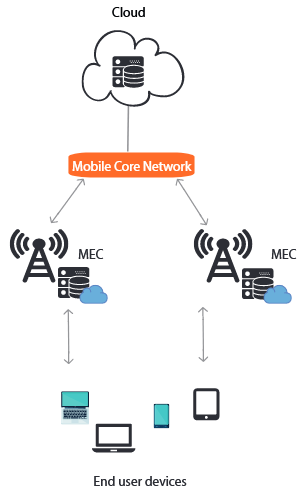
\includegraphics[width=0.3\textwidth]{./images/4/MEC.png}
    \caption{General architecture of edge computing\cite{MobileEdgeComputing}}
    \label{fig:mec}
\end{figure}

There are already some companies offering \acrfullr{saas} solutions for edge computing, but there are open solutions that can be integrated in a edge node to create a middleware for the system. One of this 
technologies is the \texttt{Thingsboard} platform. This platform\cite{ThingsBoardOpensourceIoT} allows for:
\begin{itemize}
    \item Device management.
    \item Data aggregation.
    \item Data collection.
    \item Data processing.
    \item Visualization solutions or piping to other services.
    \item Intercommunication interfaces.
    \item Scalability.
    \item Integration with other useful technologies like \texttt{Kafka} for logs or \texttt{Node Red} for simulation of events.
\end{itemize}
